\chapter{Background} \label{background}
Since this project is largely focused around designing and building a new hardware architecture,
it is necessary to go through the existing material surrounding this topic. Hardware design can
be structured in many different ways. For the purposes of this report, a structuring based on increasing
abstraction levels will be used. Since the implementation objectives of the project aim to be educational in nature,
it is crucial to start off with as few assumptions about the existing systems as possible. As such, the following explanations assume zero previous knowledge. Besides this, the educational outcomes largely focus on developers and computer scientists, professionals who would benefit from a better understanding of the computer but who are not necessarily familiar with the field of logic design. As such, the definitions and explanations will be kept as brief as possible, to avoid possibly superfluous levels of detail.

\section{Computer Architecture}
Computer architecture refers to organization, functionality and implementation design details of a computer system. It can be generally split into two main categories: \emph{Instruction Set Architecture} and \emph{Microarchitecture}.

\subsection{Instruction Set Architecture (ISA)}
The \emph{Instruction Set} is the set of unique operations the computer is capable of performing. It is generally independent of the physical implementation of the system and it serves as an interface against which assembler, compiler and operating system designers and engineers can structure their products. ISA design will be a crucial part of this project. By building a hardware architecture from scratch, the opportunity for many different ISA design choices will present itself. Many of those choices will be presented, implemented and analysed in this report.

\subsection{Microarchitecture}
A computing system's microarchitecture refers to concrete and detailed implementation choices for the hardware which is to implement the Instruction Set defined through the ISA. For the purposes of this project, the microarchitecture design will come first, which will be done against a general set of requirements and then the ISA design will follow based on the hardware design choices made. The ISA design will serve as a stepping stone towards the software architecture stage of the project.

\subsection{General High-Level Architecture}
Generally speaking, all computers share some high-level design features:
\begin{itemize}
  \item \emph{A Processor,} or \emph{Arithmetic-Logic Unit (ALU),} which performs operations on some data
  \item \emph{A Memory} or \emph{Storage Unit,} which stores both data and instructions
  \item \emph{A Control Unit,} which decodes instructions and issues control signals
  \item \emph{Input/Output (I/O) devices,} to communicate with the outside world
  \item \emph{A Clock Pulse Generator,} which keeps all other modules running synchronously
  \item \emph{A Data Bus,} to facilitate the transfer of information between modules
\end{itemize}
Each individual component will be discussed in great detail in this report.

\begin{figure}[H]
  \centering
  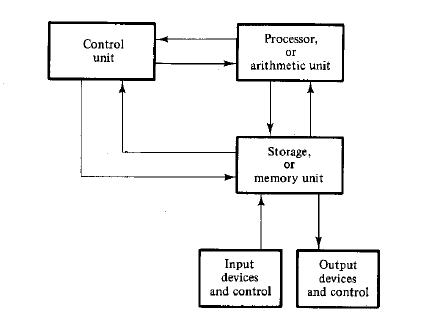
\includegraphics{comp_architecture}
  \caption{Block diagram of a digital computer, adapted from \emph{Digital Logic and Computer Design} by M. Morris Mano \cite{mano2017digital}}
  \label{comp_architecture}
\end{figure}

Figure \ref{comp_architecture} is a block diagram based on the previous listing of modules. The Data Bus is represented as the double-ended arrows connecting the different components together. The clock is omitted.

\subsection{The Processor}
The processor module is tasked with executing certain operations on data. Its mode of operation is only dependent on two inputs: the data to be operated on and the operation to be applied to that data. As such, the processor does not have to hold any kind of internal state; its output will always be the same for a certain input. This makes the processor a \emph{combinatorial circuit}, meaning that it just implements some (albeit complex) logic function and does not have any internal state or memory.

\subsection{Memory}
Memory serves the purpose of storing data and instructions and returning the stored information when requested. By nature, it is a \emph{sequential} circuit, meaning that it has some internal state besides the logical function implementations used to communicate with the rest of the computer. Memory is organized in addresses, each address storing a word of information.

\subsection{The Control Unit}
The Control Unit oversees all other modules and ensures that everything is happening according to the present instruction. It also has the task of decoding the present instruction to correctly select the control signals which have to be issued next.
There are two main design choices to be made when constructing a Control Unit. One option is to \emph{hardwire} the logic. Whilst more efficient, this often proves to be tedious and very hard to alter. Another common and more accessible approach is the use of \emph{microcode.} Microcode control units use some sort of \emph{Read-Only Memory (ROM)} as a \emph{lookup table} to decide which control signals to switch on at a given time step of a given instruction. This lookup table is microcode. As it is implemented through a ROM, it can be easily reprogrammed or swapped out for a different ROM, making the maintenance of the Control Unit much more accessible.

\subsection{Input/Output Devices}
Input devices are used to inject instructions and data into the computer. Output devices communicate calculated results back to the user. I/O devices can take many forms and usually also require the computer to implement some sort of \emph{interrupt} system to notify the control logic that an external event is taking place. In the case of the computer built for this project, I/O devices will be abstracted as simple registers. The computer will read from and write to those registers.

\subsection{The Clock Pulse Generator}
Computers rely on a master clock to synchronise the activity of all other components. In modern microcomputers, this is usually accomplished through a \emph{crystal osscilator} which vibrates at a predetermined frequency. There are also other ways to achieve a steadily pulsating clock signal. In the case of the computer built in this report, a pair of voltage comparators will be used.

\subsection{The Data Bus}
Given a large number of modules present in a computer, it comes off as impractical to have each module communicate with each other module directly. In this situation, the data bus presents itself as an adequate solution. All modules connect both their input and their output terminals to the bus through some guard or buffer which allows them to disconnect from the bus as needed. Then, at any given clock pulse, only one device is allowed to connect and output to the bus, whilst any devices interested in receiving that information can connect and input from the bus. As long as only one device writes to the bus per clock cycle, the bus functions properly.

\subsection{Other Important Components}
Besides the main modules listed above, there are a few more components which are crucial to the optimal operation of a computer.

\subsubsection{Registers}
Registers are small memory units which can store only one word of memory. A computer system normally has a very limited amount of registers. In modern computers, registers have much shorter access times than memory. Besides storing data and programs, registers can have special functions, for example, input and output registers, registers tied to certain operations, flags registers and instruction registers.

\subsubsection{Power Supply}
Since the focus of this project is electrical computers, some sort of electrical power supply will be necessary. A simple solution for a power supply based on a standard ATX power supply will be presented in a later section of the report.

\section{Implementing individual modules}
With the general architecture of a computer system in place, the next design step is to create and implement designs for each individual module. This can be achieved by using circuit design theory and best practices, which are the ~~tools'' in the circuits designer's ~~toolbox''. An in-depth analysis of these can be found in the Appendix section of the report.


\section{8-Bit Computer Architecture Implementation by Ben Eater \cite{eater2019breadboard}}
This section concerns itself with the detailed analysis of the 8-bit computer architecture implemented by Ben Eater in his YouTube tutorial series \cite{eater2019breadboard}. This computer serves as the starting design for the computer discussed in this report in the later section, as such, it presents itself as a good topic for discussion.

\subsection{Main Features}
The main features of Bean Eater's 8-bit computer on a breadboard can be broken down as follows:
\begin{enumerate}
  \item 16 by 8 memory space (4-bit addresses, 8-bit words)
  \item adjustable and manually single-steppable clock
  \item two data registers: A and B
  \item ALU which implements addition, subtraction and simple branching based on zero and carry conditions
  \item Decimal output through three 7-segment displays
  \item Microcode-based control logic using \emph{EEPROMs} (electronically erasable and programmable read-only memory)
  \item Common 8-bit data and instruction bus
\end{enumerate}

\subsection{High-Level Overview}
\begin{figure}[ht]
  \centering
  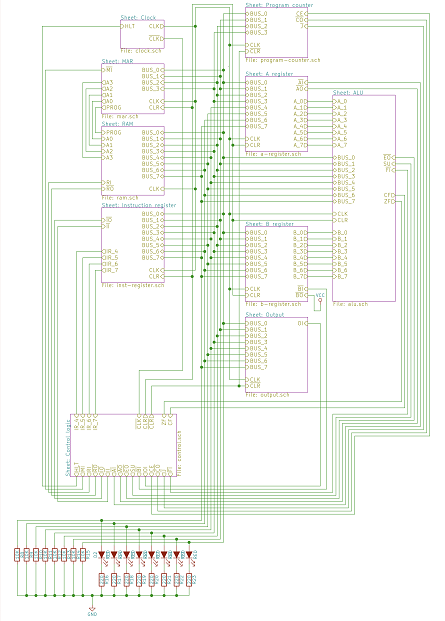
\includegraphics{8-bit-high-level}
  \caption{Block diagram of the 8-bit computer built by Ben Eater \cite{eater2019highlevel}}
  \label{8-bit-high-level}
\end{figure}



Figure \ref{8-bit-high-level} is a high-level block diagram displaying the inner workings of the 8-bit computer built by Ben Eater\cite{eater2019breadboard}. The following observations can be made when observing this diagram:
\begin{enumerate}
  \item Each module is connected directly to the common data bus. This means that every module can output information to the bus each clock cycle. After a judicious inspection of the microcode\cite{eater2019microcode} it is clear that no two modules output to the bus at the same time.
  \item The clock signal and the inverse clock signal are distributed throughout the computer to each module. Also, notice how there is a control signal for the clock as well. This \emph{HLT} (Halt) signal allows the computer to halt the clock, and implicitly halt the execution, for example after finishing a calculation, to allow it to be displayed.
  \item Besides the main connections through the bus, there are some additional \emph{special connections} between certain modules. For example, the \emph{A register} and the \emph{B register} have a direct connection to the \emph{ALU}, the \emph{MAR} (Memory address register) has a direct connection to the \emph{RAM} (Random Access Memory) and the \emph{IR} (Instruction Register) has a direct connection to the control logic.
  \item All control signals originate from the \emph{Control Logic} and spread out throughout the computer. Each module has at least one control signal
  \item This computer is severely limited in terms of memory. While 16 bytes can be sufficient for some demonstrational trivial programs (like Factorial or Fibonacci), it is insufficient for anything else.
  \item Another major limitation is the fact that it can only operate on signed integers. The architecture represents data in \emph{big endian, two's complement integer} format. No other data format or type is supported.
\end{enumerate}

\subsection{Module Design Conventions}
Ben Eater follows some essential design conventions when designing and building each of the modules for his computer.
The following subsections describe those conventions.

\subsubsection{Simplicity of understanding over cost and efficiency}

In many situations where a simpler solution from cost or efficiency makes itself notices, Eater often chooses to go for a more pragmatical approach which focuses on the simplicity of understanding. Since his computer mostly serves as an educational tool, it makes sense to pursue solutions which are easy to understand, over solutions which might be slightly cheaper or more efficient. A good example of this is in the design of the clock module \ref{8-bit-clock}.

\begin{figure}[ht]
  \centering
  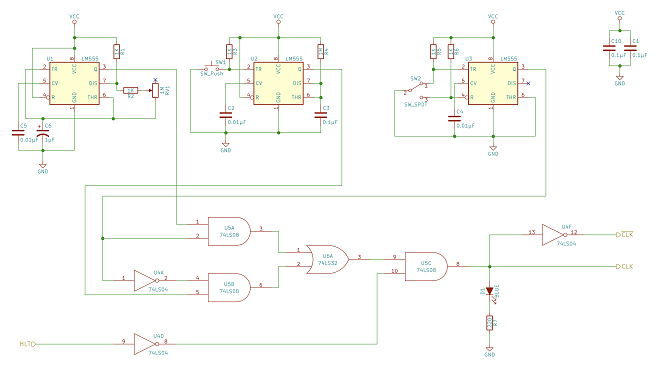
\includegraphics{8-bit-clock}
  \caption{Schematic of the clock module in Bean Eater's 8-bit computer \cite{eater2019highlevel}}
  \label{8-bit-clock}
\end{figure}

For the combinatorial circuit responsible for selecting a clock signal (either the automatic or the manual one) and also filtering out the clock when the \emph{HLT} (Halt) signal is active, Eater could have opted for a circuit built out of \emph{NAND} (Not And) gates instead of a circuit of AND, OR and inverter gates. This is because NAND gates are universal gates, which means that any combinatorial circuit can be built exclusively out of NAND gates. In this case, this would have had a net effect on cost, since the circuit could have been implemented with only two NAND ICs (integrated circuits), instead of three. The choice was made to use AND, OR and Inverter gates since the function of those gates is more intuitive and as such, the entire circuit is easier to understand.

\subsubsection{Connection to the Bus}

Eater's computer features an 8-bit common bus for both data and instructions. Most modules are tied to this bus directly. For the bus to function properly, only one device should be allowed to output to the bus at a time. Without some guards, connecting to the bus directly would mean that all modules would inadvertently drive the bus either high or low, depending on their output. The solution to this is the use of \emph{Tri-State buffer gates.} This gates can be set to be in three states, either on or off, depending on the signal passing through them, or in a \emph{high-impedance} state in which the two terminals of the buffer are essentially disconnected from each other. This is activated through a separate control signal. All modules which output to the bus do so through an IC (integrated circuit) containing such gates. An example of this can be seen on the A register \ref{8-bit-a-register}.

\begin{figure}[ht]
  \centering
  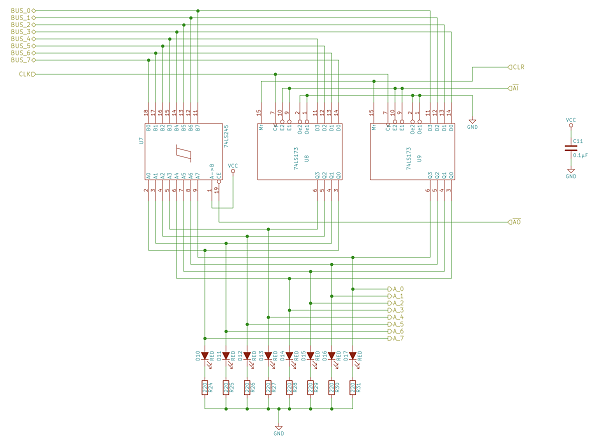
\includegraphics{8-bit-a-register}
  \caption{Schematic of the A register in Bean Eater's 8-bit computer \cite{eater2019highlevel}}
  \label{8-bit-a-register}
\end{figure}

\subsection{Analysis Conclusions}
Based on the previous analysis we can draw the following conclusions about Eater's approach towards implementing SAP-1:

\begin{itemize}
  \item When faced with a choice between efficieny/cost or simplicity, simplicity should always be chosen, since the purpose of the build is academic/educational in nature.
  \item Each module of the computer should follow the following pattern: data inputs and outputs come and go from the common bus,
  while control signals come directly from the \emph{Control Logic} module.
  \item Each module should execute one function and do it well. This is very similar to the Unix Programming Philosophy.
\end{itemize}

Taking all of these finding into account, the next step is to set out the specifications for the enhanced computer which is to be built in this report and then come up with designs matching those specifications.
